\documentclass[conference]{IEEEtran}
\IEEEoverridecommandlockouts
% Revision of main.tex from the supplied chainguard_isl.zip (main.tex only).
% Prepared 9 October 2026; implementation/results snapshot: 8 October 2026.
% Architecture Lock v1.1 unchanged. Results were not rerun for this revision.
\usepackage{cite}
\usepackage{amsmath,amssymb,amsfonts}
\usepackage{graphicx}
\usepackage{textcomp}
\usepackage{xcolor}
\usepackage{array}
\usepackage{booktabs}
\usepackage{hyperref}
\hypersetup{colorlinks=true, linkcolor=blue, urlcolor=blue, citecolor=blue}

\def\BibTeX{{\rm B\kern-.05em{\sc i\kern-.025em b}\kern-.08em
    T\kern-.1667em\lower.7ex\hbox{E}\kern-.125emX}}

% Vector PDF companions use the existing graphicx package without SVG build-time conversion.

\begin{document}

\title{ChainGuard: Retained-History Representations and Verifiable Evidence for MCP Workflows}

\author{
\IEEEauthorblockN{Saanvi Bansal\textsuperscript{1}, Aryan Malik\textsuperscript{2}}
\IEEEauthorblockA{
Dept. of Computer Science Engineering \\
Manipal Institute of Technology, Manipal Academy of Higher Education \\
Manipal, India \\
\textsuperscript{1}240953564, \textsuperscript{2}240953668}
}

\maketitle

% SOURCE: Lock §§6,15--20; Results Ledger ENG-* and Phase 2;
% chainguard/{client,proxy,detectors,oracle,audit,evidence,verifier,acceptance,workflows}.py.
\begin{abstract}
ChainGuard is a controlled Model Context Protocol (MCP) testbed for studying how retained historical information affects deterministic security decisions. It compares current-event features (B0), an unordered historical projection (B1), and ordered stateful evaluation (B2), while separately examining evidence integrity, decision reproduction, and expected-run acceptance. This Evaluation-1 report documents supported local MCP mediation, replay-based representation checks with an independent oracle, durable SQLite persistence, SHA-256 hash-chained evidence with ECDSA P-256/SHA-256 closure, and offline verification and acceptance. Recorded qualification comprises 216 passing automated tests across separately executed suites. A real non-release demonstration produced 26 audit records in eight confirmed transactions; offline inspection passed six dimensions and reproduced 12 findings. Adversarial review exposed a persistence-gate weakness and motivated exact persisted-batch verification before commit, trusted-state advancement, and forwarding. These are bounded engineering results. Live release-permission lifecycle validation, external comparison, held-out evaluation, and final performance measurements remain pending; when ordered history improves useful security decisions remains an empirical question.
\end{abstract}

\begin{IEEEkeywords}
Model Context Protocol, retained history, deterministic policy evaluation, independent oracle, audit evidence, ECDSA, expected-run acceptance
\end{IEEEkeywords}

\section{Introduction}
% SOURCE: MCP basic specification; Wang primary paper.
MCP provides a structured interface through which AI applications interact with external tools and resources~\cite{mcp2026}. Security decisions at this interface may depend on facts retained from earlier operations. Contextual enforcement already appears in prior MCP security research~\cite{wang2026}; the relevant question is which historical information a particular policy requires, rather than whether all existing defenses examine calls independently.

% SOURCE: Lock §§6,16; Project Charter research questions.
ChainGuard studies three representations under fixed controlled semantics: B0 observes the current event, B1 adds unordered historical facts, and B2 evaluates ordered state. B1 separates the value of retaining history from the value of preserving order. Persistent exposure to a sensitive source can be represented without event order, whereas revocation and subsequent regrant can require distinctions that counts alone discard~\cite{cglock}.

% SOURCE: Lock §§8--10,19; Claims Register MET-01/SEC-01--03.
Evaluation also requires evidence whose integrity, origin, context, and reproducibility can be checked. ChainGuard separates durable capture, authenticated closure, offline finding reproduction, and whole-run acceptance. None establishes observation truth merely by authenticating evidence. This report presents the completed Evaluation-1 engineering slice, reserving comparative empirical conclusions for the final study~\cite{cgresults,cgprotocol}.

\section{Problem Statement and Objectives}
% SOURCE: Lock §§4,6,15--20; Charter RQ1--5.
The problem is to assess how current-event, unordered-history, and ordered-state representations affect deterministic decisions for bounded MCP workflows, while preserving independently inspectable evidence. Contract authorization, behavioral warnings, execution effects, and evidence status must remain distinct. Detector recommendations must also be distinguished from common-controller refusals~\cite{cglock,cgprotocol}.

% SOURCE: Lock §20; Results Ledger ENG-M1--M5.
The measurable current objectives and their evidence are:
\begin{enumerate}
\item \textbf{O1: Demonstrate supported MCP mediation.} Correlated discovery, tool listing, and success/error/success calls establish the configured client--proxy--server path (M1).
\item \textbf{O2: Implement and compare B0/B1/B2 under controlled fixtures.} Frozen projections, prewritten oracle expectations, matched B1 inputs, and B2-R/B2-S agreement establish replay qualification (M2 and Phase 2).
\item \textbf{O3: Persist and independently verify committed audit evidence.} Transaction-gate fault checks and separate-process verification establish persistence, signed closure, and finding reproduction (M3/M4).
\item \textbf{O4: Implement expected-run acceptance and duplicate rejection.} Fresh acceptance, rejection after verifier restart, and inventory/concurrency checks establish the bounded submission contract (M5).
\end{enumerate}
These objectives map to engineering evidence~\cite{cgresults}; they imply neither a project completion percentage nor completion of the final research study.

\section{Related Work}
% SOURCE: Deng arXiv:2406.02630v2/CSUR metadata; Hou arXiv:2503.23278v3.
Deng \emph{et al.}~\cite{deng2025} organize agent-security concerns around input sequences, internal execution, operating environments, and external interactions. Hou \emph{et al.}~\cite{hou2026} examine MCP architecture and security across the server lifecycle. These surveys motivate explicit observation boundaries, but do not establish that ordering is necessary for every tool-security policy.

% SOURCE: verified MDPI Electronics 15(13),2829; Lock §17; Baseline Notes.
Wang \emph{et al.}~\cite{wang2026} interpose a policy enforcement point at the tool-call boundary, propagate source-integrity and data-sensitivity labels across trace steps, and record decisions in a SHA-256-linked log. This relevant prior work invalidates a general claim that MCP defenses lack session context. It is a planned external comparison target, not an implemented ChainGuard baseline. The locked comparison is limited to a conformance-tested sensitivity-policy subset using common facts, rather than complete external-system reproduction~\cite{cglock,cgprotocol}.

% SOURCE: AgentSpec arXiv:2503.18666v3; CaMeL arXiv:2503.18813v2.
AgentSpec~\cite{agentspec} expresses structured runtime constraints through triggers, predicates, and enforcement actions. CaMeL~\cite{camel} separates control and data flows and uses capabilities to constrain tool-mediated disclosure. These approaches provide precedents for runtime policy and agent/tool authorization. ChainGuard's coarse historical-exposure rule does not establish equivalent data-provenance or information-flow guarantees~\cite{cgthreat}.

% SOURCE: verified MDPI Applied Sciences 16(15),7662.
Spotlight-Guard~\cite{demirol2026} combines isolation of untrusted content, model-based detection and quarantine, and HMAC instruction-integrity checks. This layered design provides context for separating behavioral defenses from integrity mechanisms. ChainGuard evaluates deterministic controlled policies and public-key authentication of committed audit evidence; the external paper's metrics are not results of this project.

% SOURCE: RFC 5848; FIPS 186-5; Lock §§8--10.
Signed syslog~\cite{syslog} provides an established precedent for authenticated, sequenced logging and detection of missing messages. ECDSA is specified in the Digital Signature Standard~\cite{dss}. ChainGuard applies established mechanisms with independent trust anchors and task-bound expectations~\cite{cglock}. Combining contextual decisions and authenticated logs does not establish first-of-kind novelty.

% CITATION REVIEW TODO: singh2026 is retained as an inactive bibliography comment.
% Title conflicts with discoverable MCP-Secure metadata; primary publisher
% verification unavailable. Do not cite mechanism/performance or adopt new
% title/authors/pages/DOI until the owner checks the primary paper.

\section{Research Gap and Scope}
% SOURCE: Claims MET-01/EMP-01--05/NOV-01; Lock §§6,16,20.
The bounded gap is a controlled characterization of how current-event, unordered-history, and ordered-state representations affect decisions for specified MCP workflows, alongside separate evaluation of evidence integrity, reproduction, and acceptance. The engineering contribution is the working testbed and qualified evidence pipeline. The research question concerns conditional decision quality and task effects; held-out validation and external comparison are future empirical work~\cite{cgprotocol,cgresults}.

% SOURCE: Lock §§3--4,16--20; README M1/M2/M4; Claims SEC-04/05.
Current scope is local stdio mediation with scripted clients and controlled tools. Sensitive-release and scoped-authorization semantics are exercised in replay; the integrated live demonstration uses public, non-release calls. Grant, scope-revocation, and one-use consumption remain mandatory final capabilities despite unfinished live M6 validation. Arbitrary MCP servers, other transports, general information-flow tracking, and real-LLM prompt-injection robustness are outside demonstrated coverage~\cite{cglock,cgresults}.

\section{Threat Model}
% SOURCE: THREAT_MODEL actors/adversaries/assumptions; Lock §§3--5,15,18.
ChainGuard mediates supported calls routed through its configured proxy. The trusted host establishes task identities and execution permissions; client metadata cannot create grants or reset context. The monitor, normalizer, controlled registry/tools, verifier, and assessor runtime are trusted within the experiment. Protected assets include synthetic sensitive data, scoped permissions, task state, audit commitments, keys, expected inventory, and acceptance state~\cite{cgthreat}.

% SOURCE: Threat Model evidence-storage attacker; Lock §§8--10,19.
The simulated storage attacker may alter SQLite records or exported packages, recompute unkeyed chains, substitute bundle-supplied configuration, or resubmit authentic evidence. Signing keys, trusted running state, external verifier pins/configuration, independent oracle journals, and the durable acceptance registry remain outside that authority. Storage cannot become the authority for recovering running permission or commitment state. These are logical boundaries, not demonstrated operating-system privilege isolation~\cite{cgthreat}.

% SOURCE: Threat Model workflow attacker/limits; Lock §§15.2,18,19.
The workflow attacker may arrange valid controlled calls and arguments but cannot issue trusted controls or bypass the mediated path within the experiment. The oracle assesses pre-decision authorization and independently observes dispatch, consumption, covered disclosure, and completion; it does not authorize execution. Host/key compromise, registry rollback, unsupported leakage, and unmediated actions are outside coverage. Local timestamps provide display context, not trusted time~\cite{cgthreat,cglock}.

\section{System Architecture}
% SOURCE: Lock §2,15--19; proxy.py/run; audit.py/LiveAudit; m3.py/shadows;
% evidence.py/ChainedAuditSession; verifier.py; acceptance.py.
The core path connects the MCP client to the stdio proxy and controlled server. The proxy correlates proposals and outcomes; current facts and eligible history feed B0/B1/B2. The controller owns execution authority, persists proposal/decision/dispatch intent, and permits forwarding only after the audit gate succeeds. Outcomes are persisted separately. Independent fixture/environment observations feed the oracle on a separate path to experimental labels~\cite{cglock}.

\begin{figure*}[t]
\centering
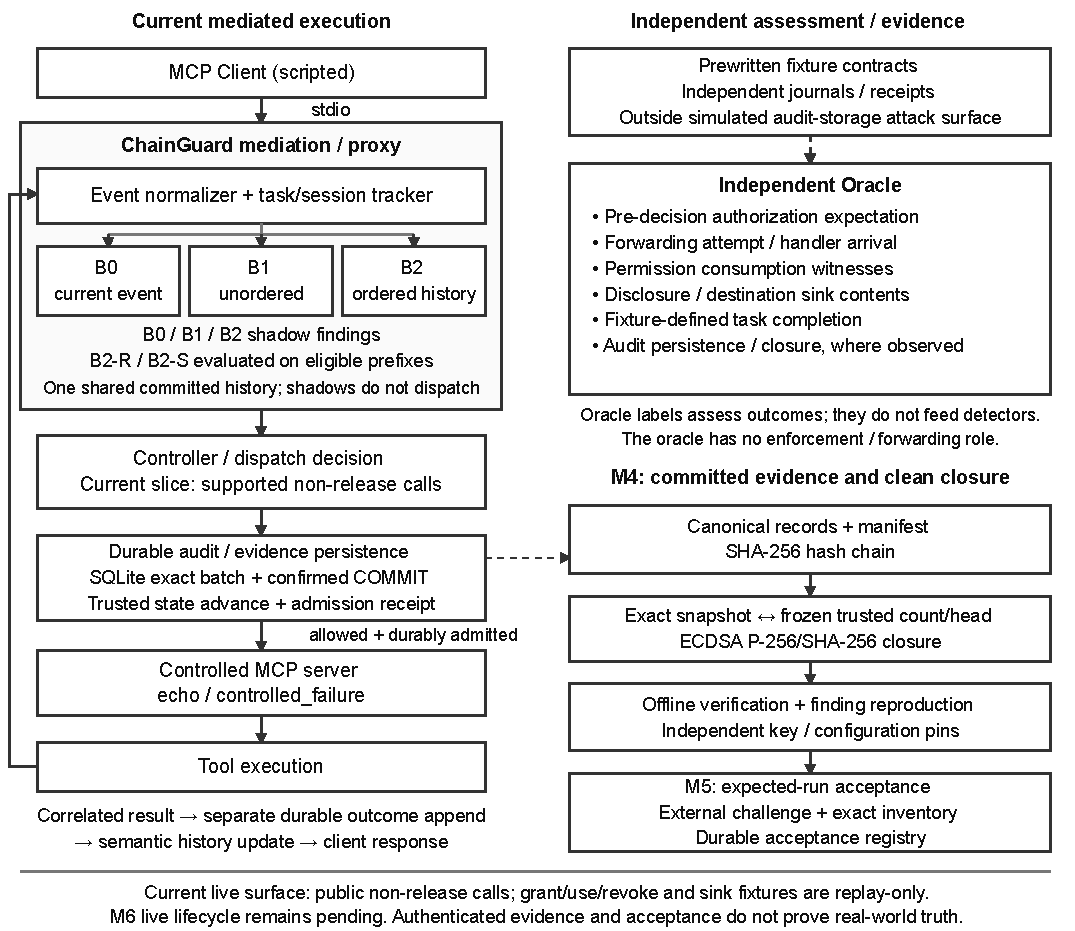
\includegraphics[width=\textwidth,height=0.74\textheight,keepaspectratio]{figures/fig1_architecture.pdf}
\caption{ChainGuard system architecture showing MCP mediation, representation-specific evaluation, durable evidence persistence, independent oracle observations, and downstream verification.}
\label{fig:architecture}
\end{figure*}

% SOURCE: canonical.py; evidence.py/event_hash,seal; verifier.py/DIMENSIONS;
% acceptance.py/submit; Lock §§8--10,19.
The evidence path converts audit records into restricted canonical JSON, links them with domain-separated SHA-256 hashes, and authenticates closure using ECDSA P-256/SHA-256. Offline verification uses externally trusted keys/configuration to inspect frozen evidence and reproduce findings. Acceptance adds independently retained context, exact inventory, and a durable registry. Figures~\ref{fig:architecture} and~\ref{fig:evidence} show the architecture and evidence path~\cite{cglock}.

\section{Methodology}
% SOURCE: Lock §§6,15.3,16; semantics.py/Fact,Bucket; protocol representations.
The representations share current normalized proposal $c_t$, static policy, and controlled semantics. Eligible history $H_t$ contains only prior tool outcomes, grants, scope revocations, and once-only USE facts projected from committed dispatch intent. Findings, controller conclusions, audit bookkeeping, and future results are excluded. M2 commitments are staged fixture assumptions, not live persistence proof~\cite{cglock,cgprotocol}.

% SOURCE: Lock §§15.2,15.4; protocol attribution.
Shadows evaluate one controller-generated history without controlling dispatch or consuming grants. Normal observation does not bypass authorization. Unauthorized forwarding requires an explicitly configured, default-disabled synthetic local-sink override committed in the controller profile; static prohibitions and persistence failures still block. Enforcement comparisons require separate executions, with controller refusals attributed separately~\cite{cglock,cgprotocol}.

\subsection{B0 Current-Event Representation}
% SOURCE: semantics.py/extract_current,B0_OPERATING_POINT; detectors.py/b0; Lock §16.
B0 receives current-event features only. Frozen direct recognition checks registered synthetic canaries in raw UTF-8 or one strict base64 layer and applies static destination restrictions. Historical exposure and active-grant state are unavailable. Missing historical authority is INDETERMINATE: a hypothetical ALLOW recommendation without current warnings does not establish task authorization. This is a meaningful bounded per-call operating point~\cite{cgprotocol}.

\subsection{B1 Unordered Historical Representation}
% SOURCE: semantics.py/Bucket,project_b1; detectors.py/b1; Lock §16.
B1 retains counts by category, operation, resource, destination, outcome, sensitivity, transformation, and exact release scope. It removes order, timestamps, event/grant IDs, predecessor links, active-state flags, and transitions, while retaining successful exposure. For scope $s$, let $G_s$, $R_s$, and $U_s$ denote grant, revocation, and use counts. Under validated lifecycle, permission holds when $G_s>U_s$ and $R_s=0$; absence holds when $G_s\leq U_s$; $G_s>U_s$ with $R_s>0$ is INDETERMINATE. Conservative denial of required uncertain permission records SUSPICIOUS rather than a definite violation~\cite{cglock}.

% SOURCE: Lock §16; protocol E02; test_workflows.py matched-input tests.
B1 isolates historical information from ordering information (Figure~\ref{fig:representations}). Matched-order cases require byte-identical serialized B1 inputs and independent labels; equal event totals alone are insufficient. Mixed-label groups demonstrate ambiguity for observed inputs, not a theorem about all unordered representations~\cite{cgprotocol}.

\subsection{B2 Ordered Stateful Representation}
% SOURCE: detectors.py/B2Reference,B2Streaming,equivalent; m3.py/shadows; Lock §16.
B2 evaluates ordered exposure and grant/revoke/use transitions. Revocation invalidates active matching grants; a later new grant may restore permission. Failed/denied acquisition creates no exposure, and committed-intent consumption is not refunded after dispatched failure. B2-R reconstructs the full eligible prefix; B2-S applies incremental transitions. Agreement on assessments, verdicts, recommendations, rules, and deterministic references is implementation consistency, not independent correctness. The live callback rebuilds its streaming evaluator from the prefix and therefore establishes no retained-state scaling result~\cite{cglock,cgprotocol}.

The lifecycle pair in Figure~\ref{fig:representations} is illustrative, not an executed empirical result; independent fixture/oracle labels determine whether the resulting distinction is correct.

\begin{figure*}[t]
\centering
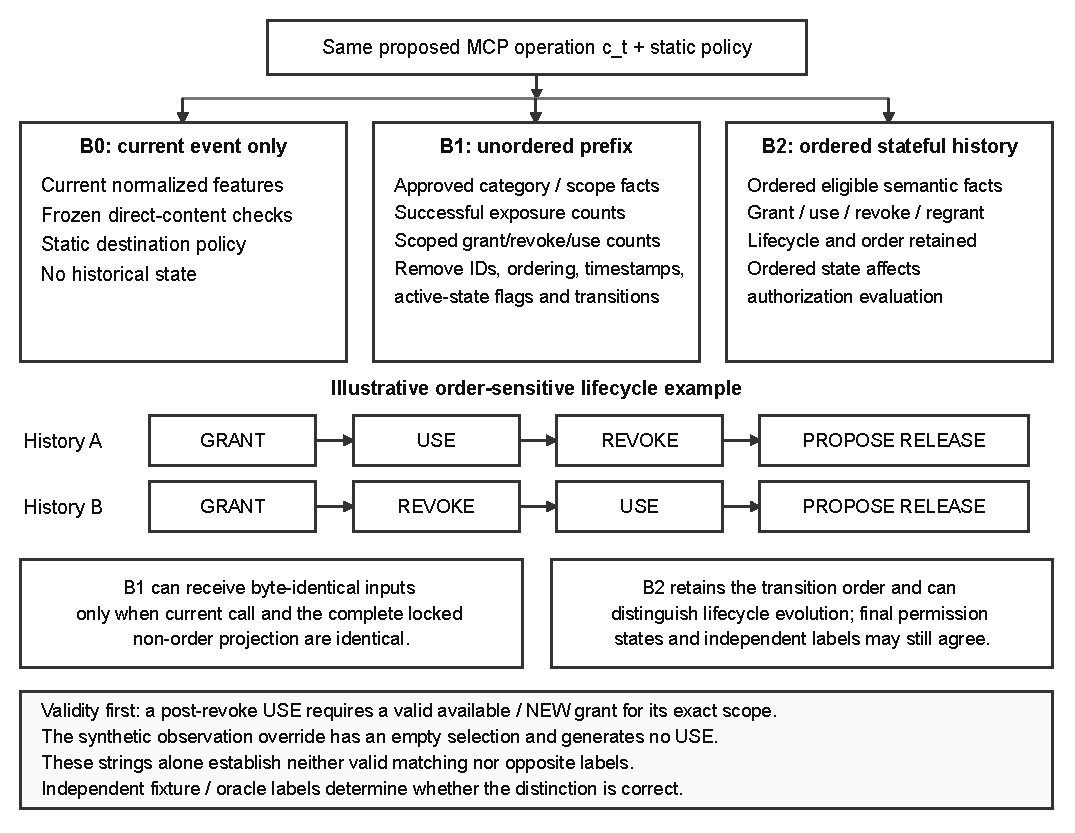
\includegraphics[width=\textwidth,height=0.74\textheight,keepaspectratio]{figures/fig2_b0_b1_b2.pdf}
\caption{Comparison of current-event, unordered-history, and ordered-state representations used by ChainGuard.}
\label{fig:representations}
\end{figure*}

\subsection{Independent Oracle}
% SOURCE: oracle.py imports/assess; workflows.py/qualify; Lock §18; protocol Phase 2.
The oracle reconstructs the written contract from assessor-held raw journals and observations without importing detector or normalizer transitions. It assesses authorization before each decision, including denial. Dispatch, consumption, destination-tagged canary disclosure, and completion remain separate. Missing witnesses preserve UNKNOWN/INDETERMINATE; findings or audit closure cannot replace them. Phase-2 receipt structures currently use injected synthetic observations and staged authorization journals, without a qualified live collector~\cite{cgprotocol,cgresults}.

\subsection{Audit and Evidence Pipeline}
% SOURCE: audit.py/append_batch,_validate_storage_schema,_verify_stored_batch;
% evidence.py/_verify_stored_batch,seal; proxy.py/run; AF-001.
The allowed-call invariant is proposal $\rightarrow$ decision $\rightarrow$ dispatch intent $\rightarrow$ SQLite transaction $\rightarrow$ exact persisted-batch verification $\rightarrow$ confirmed COMMIT $\rightarrow$ trusted-state advancement $\rightarrow$ forwarding. Readback occurs inside the transaction before COMMIT against frozen expected rows, with code-owned schema and M4 manifest checks. Persistence failure blocks forwarding; ambiguous execution commit halts without adopting database state or retrying tools~\cite{cgresults,cglock}.

% SOURCE: canonical.py; evidence.py/manifest_digest,event_hash,seal; verifier.py.
Canonicalization constrains types and encoding. Closure freezes trusted manifest digest, count, and chain head; the exporter reconciles an exact snapshot, signs through the reviewed library, and self-verifies. Offline checks separately report structure, commitment integrity, trusted signature, expected binding, completeness, and finding reproduction. Authentication and reproduction do not establish raw observation truth~\cite{cglock,cgthreat}.

\begin{figure*}[t]
\centering
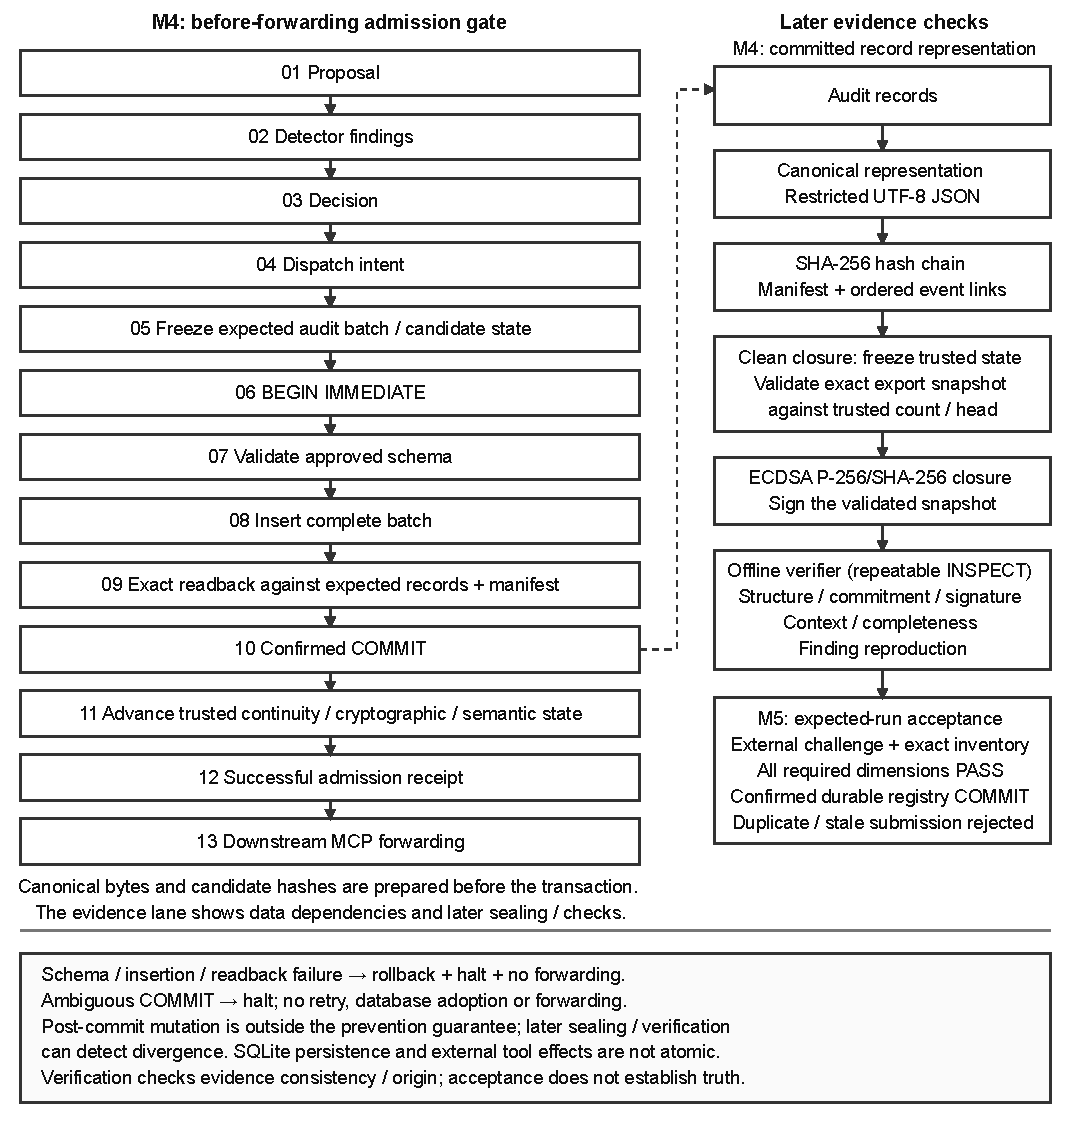
\includegraphics[width=\textwidth,height=0.74\textheight,keepaspectratio]{figures/fig3_evidence_flow.pdf}
\caption{Durable audit and evidence flow, including the pre-forwarding persistence gate and subsequent verification and acceptance stages.}
\label{fig:evidence}
\end{figure*}

\subsection{Expected-Run Acceptance}
% SOURCE: acceptance.py/register,submit; verifier.py/inspect_run; Lock §19.3.
Before execution, the assessor retains expected run/challenge, exact task/session/monitor inventory, configuration, and signer pins independently of the package. M5 requires every expected session exactly once and all required dimensions PASS. A durable transaction rechecks ACTIVE state, records authenticated commitments, and transitions the whole run to ACCEPTED. Acceptance follows confirmed commit. Duplicate identity uses authenticated run/challenge/inventory, not signature bytes. Repeat inspection is permitted, and eligible evidence may record violations~\cite{cglock,cgresults}.

\section{Implementation Progress}
% SOURCE: Results Ledger Phase 2 aggregate; Lock §20.
M1--M5 form the locked minimum Evaluation-1 engineering slice. Table~\ref{tab:milestones} summarizes regression/qualification evidence; ``Complete'' applies to the stated engineering scope. Phase 2 adds the workflow/oracle foundation. These statuses imply neither final-project completion nor a justified percentage; student verification and presentation remain separate requirements~\cite{cgresults}.

\begin{table}[t]
\centering
\caption{Milestone implementation/test summary~\cite{cgresults}: engineering/regression evidence.}
\label{tab:milestones}
\small
\setlength{\tabcolsep}{3pt}
\renewcommand{\arraystretch}{1.15}
\begin{tabular}{@{}p{0.13\columnwidth}p{0.46\columnwidth}p{0.11\columnwidth}p{0.16\columnwidth}@{}}
\toprule
Gate & Functionality & Tests & Status \\
\midrule
M1 & Real MCP mediation & 12 & Complete \\
M2 & B0/B1/B2 shadows and oracle (replay) & 41 & Complete \\
M3 & Durable audit persistence & 40 & Complete \\
M4 & Cryptographic evidence and verifier & 67 & Complete \\
M5 & Expected-run acceptance & 27 & Complete \\
Phase 2 & Workflow/oracle qualification & 29 & Complete \\
\midrule
Total & Automated regression/qualification & 216 & Passing \\
\bottomrule
\end{tabular}
\end{table}

\subsection{M1---MCP Mediation}
% SOURCE: client.py/exercise; proxy.py/run; controlled_server.py; test_m1.py; README.
The SDK client launches the stdio proxy, which launches the controlled SDK server. The supported subset is discovery, tool listing, and sequential calls to \texttt{echo} and \texttt{controlled\_failure}, with correlated IDs and required per-request metadata. The target is MCP 2026-07-28; full protocol compliance and other transports are not claimed~\cite{cgresults}.

\subsection{M2---Sequence Evaluation}
% SOURCE: m2.py/ReplayLedger; semantics.py; detectors.py; oracle.py; test_m2.py.
Replay validates one synthetic journal, derives eligible history independently of shadows, and compares representations against prewritten oracle expectations. Checks include B2-R/B2-S agreement and matched B1 bytes. No tools execute and no durable commits occur; grant-bearing replay semantics do not qualify live M6~\cite{cgresults,cgprotocol}.

\subsection{M3---Durable Audit Persistence}
% SOURCE: audit.py/AuditSession,LiveAudit; m3.py; test_m3.py.
Typed SQLite batches preserve proposal, findings, decision, intent, and outcome phases. Process-owned continuity advances after successful persistence; supported non-release calls traverse the live gate. M3 records remain unsealed and non-cryptographic. The repaired shared writer checks schema and exact batch materialization before commit~\cite{cgresults}.

\subsection{M4---Cryptographic Evidence}
% SOURCE: canonical.py; evidence.py; verifier.py; m4.py; test_m4.py.
M4 creates separate hash-chained streams and signed closures, rather than authenticating old unsealed M3 history. ECDSA P-256/SHA-256 uses the installed cryptography library and an independently pinned verifier public key. Exact-snapshot reconciliation and approved installed detector code support offline inspection without tool execution~\cite{cgresults,cglock}.

\subsection{M5---Evidence Acceptance}
% SOURCE: acceptance.py; m5.py; test_m5.py; README Actual M5 validation.
M5 implements durable expected-run lifecycle and whole-run acceptance with inventory, duplicate/restart/concurrency, and atomic-update checks. Failed required evidence does not consume an ACTIVE expectation. Ambiguous registry commit reports unknown durability and requires explicit reopened reconciliation; execution-commit ambiguity instead halts without forwarding~\cite{cgresults}.

\subsection{Phase-2 Independent Workflow Foundation}
% SOURCE: workflows.py; workflow_fixtures.py; test_workflows.py; protocol Phase 2.
Nine development contracts span S1--S6: current-event/public behavior, monotone exposure, authorized release, revocation/regrant, consumption/failure/retry, and multiple resources/interleaved scopes. Contracts and independent observations are separate inputs. Qualification preserves unknowns and separates authored expectations from observed effects. It adds no live collector, held-out result, or new policy engine~\cite{cgprotocol,cgresults}.

\section{Testing and Initial Results}
% SOURCE: Results Ledger snapshot/Phase 2; README runtime versions.
These are recorded engineering results through 8 October 2026; application suites and demonstrations were not rerun for this revision. The recorded environment is Windows x64, CPython 3.14.3, SQLite 3.50.4, MCP 2.3.0, and cryptography 50.0.2. Commands and test/fixture definitions remain in the repository~\cite{cgrepo,cgresults}. Test-run durations are not latency benchmarks.

\subsection{Automated Suite Evidence}
% SOURCE: Results Ledger Phase 2 aggregate; README M5 historical discovery.
Table~\ref{tab:milestones} sums to $12+41+40+67+27+29=216$: 187 M1--M5 tests plus 29 foundation tests across separately executed passing suites. This is not a new 216-test project-wide discovery run, nor 216 independent workflows, experiments, samples, or empirical observations. The 32 package cases and 16 consolidated checks are reported separately without adding them to this total~\cite{cgresults}.

\subsection{Real MCP Mediation}
% SOURCE: README Actual M1 results; Results Ledger ENG-M1.
The recorded client command completed discovery and returned success, a controlled tool error, and success after error through the proxy. Correlated diagnostics and independent handler arrivals establish the configured path. The tool error remained a valid execution result rather than a protocol error. This demonstrates mediation and error continuity, not attack detection~\cite{cgresults,cgrepo}.
% TODO SCREENSHOT 1: actual MCP mediation terminal output, command and exit status.

\subsection{M4 Live Demonstration}
% SOURCE: Results Ledger ENG-M4-FLOW; README M4 repair; m4.py; audit.py.
The real non-release success/error/success demonstration produced 26 audit records in eight confirmed transactions. Proposals, four detector findings per proposal, decisions/intents, outcomes, and lifecycle records account for the stream. Public controlled calls demonstrate integrated mediation, persistence, and sealing, rather than live sensitive-release comparison~\cite{cgresults}.

\subsection{M4 Offline Verifier}
% SOURCE: Results Ledger ENG-M4-VERIFY; verifier.py/DIMENSIONS; README M5 validation.
Separate-process verification after monitor termination reported six PASS dimensions: schema/lifecycle/sequence, commitment/link integrity, trusted signature, expected context/configuration binding, signed/inventory completeness, and finding reproduction. Twelve findings were reproduced with B2-R/B2-S agreement at all three proposal prefixes. This establishes consistency with committed inputs and approved rules; independent oracle assessment remains necessary for observation truth~\cite{cgresults,cgthreat}.
% TODO SCREENSHOT 3: actual six-dimension M4 PASS and reproduced-findings output.

\subsection{M5 Acceptance}
% SOURCE: Results Ledger ENG-M5-FRESH/DUPLICATE/CAMPAIGN.
Fresh acceptance succeeded in one process; a new process rejected the same submission as \texttt{ALREADY\_ACCEPTED}. The declared campaign passed 32/32 package cases and 16/16 consolidated checks covering intact evidence, mutation, binding/inventory, and lifecycle/persistence conditions. These results describe the bounded engineering matrix, not arbitrary-adversary error rates or MCP execution replay prevention~\cite{cgresults}.
% TODO SCREENSHOT 4: actual fresh ACCEPTED and new-process ALREADY_ACCEPTED,
% with the same registry and authenticated run identity.

\subsection{Phase-2 Oracle Qualification}
% SOURCE: Results Ledger Phase 2; test_workflows.py independence/receipts/group tests.
The 29 foundation tests qualified nine development contracts across six strata. Independence checks use absent detector/controller imports in a fresh process, poisoned evaluators, changed findings, and receipts contradicting the plan. Missing receipt coverage remains unknown. One matched group checks identical B1-input bytes with opposite prewritten authorization labels; it is a qualification example, not a final ordering-effect estimate~\cite{cgresults,cgprotocol}.
% TODO SCREENSHOT 2: actual B0/B1/B2 comparison, oracle labels and matched inputs;
% explicitly label replay/development evidence.

\subsection{Adversarial Checks and Observed Bugs}
% SOURCE: README durability repair; AF-001; Results Ledger repair.
The persistence repair has 27 targeted passing regressions and ten independent recheck cases reported as BLOCKED. Declared admission manipulations produced no handler execution; outcome sabotage after an already audited execution halted without a false committed outcome or subsequent execution. These overlapping checks are not additional research samples~\cite{cgresults}.

Figure~\ref{fig:repair} shows the corresponding persistence-gate discovery and repair.

\begin{figure*}[t]
\centering
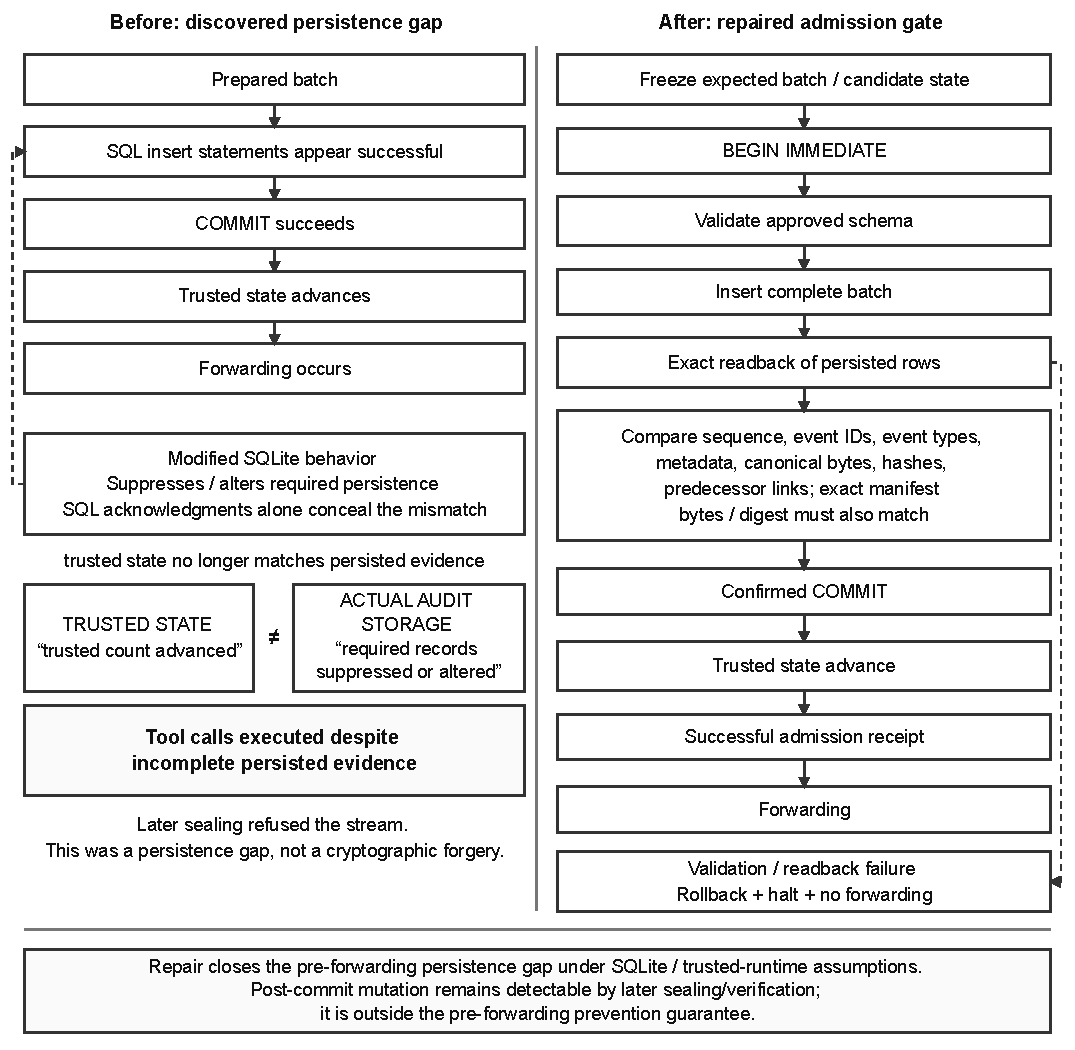
\includegraphics[width=\textwidth,height=0.74\textheight,keepaspectratio]{figures/fig4_m4_repair.pdf}
\caption{M4 persistence-gate discovery and repair: exact persisted-batch verification is required before trusted-state advancement and forwarding.}
\label{fig:repair}
\end{figure*}

% SOURCE: README Actual M2 validation; Results Ledger Phase 2 timeout.
M2 validation found an oracle bug that inferred no disclosure from task closure despite missing observations; the correction preserves unknown disclosure. Concurrent Phase-2 regression also encountered an M1 discovery timeout. An isolated unchanged rerun passed all 12 M1 tests. Subprocess load is a plausible explanation, but the root cause is not conclusively established~\cite{cgrepo,cgresults}.

\section{M4 Adversarial Discovery and Repair}
% SOURCE: ADVERSARIAL_FINDINGS AF-001; README repair; audit.py/append_batch.
The original gate treated successful SQL/transaction acknowledgment as sufficient evidence that the intended audit batch had persisted. Adversarial database behavior could suppress an expected insert while execution appeared successful. Trusted state could advance and forwarding occur without complete required evidence. Later sealing rejected the stream, but could not undo the earlier tool execution~\cite{cgresults,cgrepo}.

\begin{table}[t]
\centering
\caption{M4 persistence-gate discovery and repair (AF-001)~\cite{cgresults}.}
\label{tab:repair}
\small
\setlength{\tabcolsep}{3pt}
\renewcommand{\arraystretch}{1.15}
\begin{tabular}{@{}p{0.23\columnwidth}p{0.69\columnwidth}@{}}
\toprule
Aspect & Recorded finding / correction \\
\midrule
Assumption & Acknowledgment implied exact intended persistence. \\
Counterexample & Suppressed/altered rows despite apparently successful SQL. \\
Consequence & Trusted advancement and forwarding without the full batch. \\
Schema gate & Check tables, indexes, constraints, and temporary objects against code-owned definitions. \\
Materialization & Compare all expected metadata, bytes, hashes, and manifest before COMMIT. \\
Ordering & Confirm COMMIT, then advance trusted state and permit forwarding. \\
Boundary & No continuous protection of post-commit database contents. \\
\bottomrule
\end{tabular}
\end{table}

% SOURCE: audit.py/_validate_storage_schema,_verify_stored_batch,append_batch;
% evidence.py/_verify_stored_batch; AF-001.
The repair validates the approved schema inside the write transaction, freezes the expected complete batch, and reads back exact persisted tuples and manifest before COMMIT. Mismatch causes rollback/halt without a successful receipt, trusted advancement, or forwarding. Confirmed commit then permits state advancement and dispatch. Table~\ref{tab:repair} and Figure~\ref{fig:repair} distinguish exact materialization from acknowledgment~\cite{cgresults}.


% SOURCE: AF-001 boundary; Threat Model; evidence.py/ChainedAuditSession.seal.
The invariant assumes trusted runtime and SQLite/filesystem durability. It does not continuously protect older rows against post-commit mutation or make SQLite atomic with tool effects. Later snapshot reconciliation can refuse clean sealing on divergence from trusted count/head, but cannot reverse an executed action~\cite{cgthreat,cglock}.

\section{Current Limitations}
% SOURCE: Results Ledger B--D; Claims Register; Lock §20; protocol Phase 2/status.
M2 fixtures are primarily replay/development inputs; Phase 2 uses injected observations without a qualified live collector. M6 live grant/revoke/one-use validation remains mandatory final work. External comparison, the held-out E01--E13 study, signed-transcript comparison, and final performance/scaling measurements are unfinished. No justified overall completion percentage or final accuracy, latency, or memory result exists~\cite{cgresults,cgprotocol}.

% SOURCE: Threat Model nonclaims; protocol validity threats; Claims SEC-01--05.
Signatures authenticate committed evidence under trusted-key assumptions, not observation truth or detector correctness. Acceptance establishes submission eligibility/completeness, not benign behavior. Runtime, controlled-tool, database, and registry assumptions remain bounded. Coarse exposure can flag unrelated public transfer; unsupported decoding is outside coverage. The 216 tests are engineering evidence, not independent research observations~\cite{cgthreat,cgresults}.

\begin{table}[t]
\centering
\caption{Current evidence versus final evaluation requirements~\cite{cgresults,cgprotocol}.}
\label{tab:remaining}
\small
\setlength{\tabcolsep}{3pt}
\renewcommand{\arraystretch}{1.15}
\begin{tabular}{@{}p{0.20\columnwidth}p{0.34\columnwidth}p{0.34\columnwidth}@{}}
\toprule
Area & Current evidence & Final requirement \\
\midrule
Decisions & Replay; development contracts & Frozen held-out workflows and useful-decision analysis \\
Lifecycle & Staged grant/use/revoke & Live M6 and independent commit/effect witnesses \\
Evidence & Signed chain; reproduction & Integrity ablations, signed transcript, authentic wrong facts \\
Acceptance & Fresh/duplicate; campaign & Final case inventory and dimension-level analysis \\
Comparison & Relevant literature & Resolved pin and subset conformance \\
Cost & Test-run records only & Staged latency, memory, storage, and scaling \\
\bottomrule
\end{tabular}
\end{table}

\section{Planned Final Evaluation}
% SOURCE: Experiment Matrix E01--E13; protocol statistics; Lock §§16--20.
E01--E13 are planned experiments. E01 covers order-insensitive controls; E02 matched order-sensitive groups; E03 historical recognition outside frozen direct coverage; E04 detector/controller attribution; E05 held-out workflows; E06 live M6 lifecycle; and E07 failure boundaries. E08 requires conformance-tested external comparison. E09 examines evidence integrity, E10 authentic-but-wrong observations/findings and omissions, E11 acceptance, E12 cost/scaling, and E13 invariance/explanation~\cite{cgprotocol}.

\begin{figure*}[t]
\centering
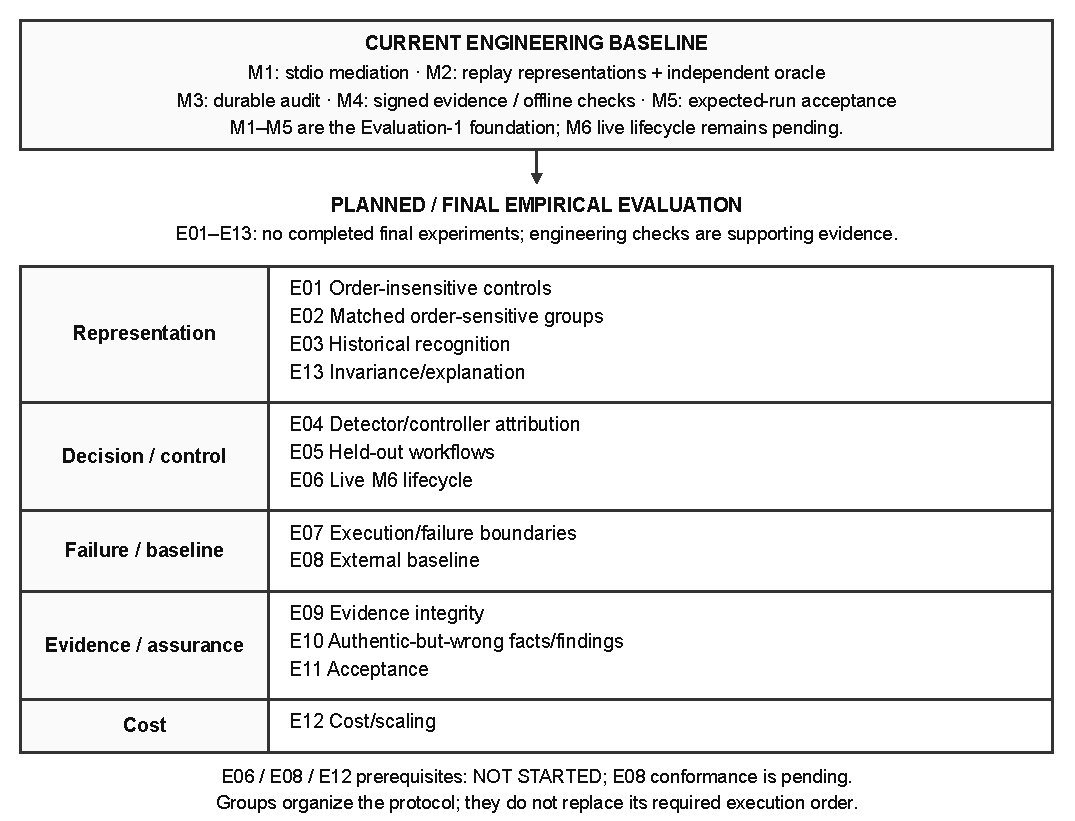
\includegraphics[width=\textwidth,height=0.74\textheight,keepaspectratio]{figures/fig5_evaluation_roadmap.pdf}
\caption{Final empirical evaluation roadmap E01--E13; these experiments are planned and are not presented as completed Evaluation-1 results.}
\label{fig:roadmap}
\end{figure*}

% SOURCE: protocol freeze/metrics; Lock §16; Baseline Notes pin ambiguity.
Policies, extraction, operating points, contracts, and parent-level splits will be frozen before held-out execution. Reporting will preserve actual independent workflow counts, eligible denominators, unknowns, completion, and detector/controller attribution. Prefixes and timing repetitions will not become independent security samples. Protocol-recorded baseline pin and evidence-label discrepancies require resolution before those experiments; the lock remains authoritative. Table~\ref{tab:remaining} and Figure~\ref{fig:roadmap} identify pending work~\cite{cgprotocol}.
% OWNER REVIEW TODO: figures/screenshots, presentation timing, live demo and viva.
% Presentation/member understanding was not observed in this revision; no marks claimed.

\section{Conclusion}
% SOURCE: Results Ledger; Claims ENG-01--05/MET-01; Lock §20; protocol status.
ChainGuard currently provides supported MCP mediation, controlled B0/B1/B2 representations, an independent workflow/oracle foundation, durable persistence, cryptographic evidence verification, and expected-run acceptance. Recorded adversarial testing identified and repaired a persistence-gate weakness. These engineering results support the bounded Evaluation-1 slice. When ordered history improves useful security decisions remains open for final evaluation~\cite{cgresults,cgprotocol}.

\begin{thebibliography}{99}
% Useful original keys retained; corrections rely only on primary sources.
\bibitem{mcp2026} Model Context Protocol, ``Basic protocol overview,'' specification 2026-07-28. [Online]. Available: \url{https://modelcontextprotocol.io/specification/2026-07-28/basic}

\bibitem{wang2026} S. Wang, S. Zhu, and R. Li, ``Runtime Policy Enforcement for MCP-Based LLM Agents,'' \emph{Electronics}, vol. 15, no. 13, Art. no. 2829, 2026, doi: 10.3390/electronics15132829.

\bibitem{cglock} ChainGuard project, ``Architecture Lock,'' ver. 1.1, Oct. 7, 2026, internal project contract, \path{docs/ARCHITECTURE_LOCK.md}.

\bibitem{cgresults} ChainGuard project, ``Results ledger,'' snapshot Oct. 8, 2026, including Phase-2 qualification, \path{docs/RESULTS_LEDGER.md}. Persistence-flaw record: \path{docs/ADVERSARIAL_FINDINGS.md}, AF-001.

\bibitem{cgprotocol} ChainGuard project, ``Evaluation protocol,'' ``Experiment matrix,'' and ``External baseline notes,'' Oct. 8, 2026, internal methodology records, \path{docs/EVALUATION_PROTOCOL.md}, \path{docs/EXPERIMENT_MATRIX.md}, and \path{docs/BASELINE_NOTES.md}.

\bibitem{deng2025} Z. Deng \emph{et al.}, ``AI Agents Under Threat: A Survey of Key Security Challenges and Future Pathways,'' \emph{ACM Computing Surveys}, vol. 57, no. 7, Art. no. 182, 2025, doi: 10.1145/3716628. Author preprint: \url{https://arxiv.org/abs/2406.02630}.

% Hou journal DOI/year from old ZIP not relied upon; primary preprint v3 inspected.
\bibitem{hou2026} X. Hou, Y. Zhao, S. Wang, and H. Wang, ``Model Context Protocol (MCP): Landscape, Security Threats, and Future Research Directions,'' arXiv:2503.23278, ver. 3, 2025. [Online]. Available: \url{https://arxiv.org/abs/2503.23278v3}

\bibitem{agentspec} H. Wang, C. M. Poskitt, and J. Sun, ``AgentSpec: Customizable Runtime Enforcement for Safe and Reliable LLM Agents,'' arXiv:2503.18666, 2025. [Online]. Available: \url{https://arxiv.org/abs/2503.18666}

\bibitem{camel} E. Debenedetti \emph{et al.}, ``Defeating Prompt Injections by Design,'' arXiv:2503.18813, 2025. [Online]. Available: \url{https://arxiv.org/abs/2503.18813}

\bibitem{demirol2026} D. Demirol and M. Aydogan, ``Balancing Security and Performance in LLM Agents: Spotlight-Guard, a Layered Defense Against Indirect Prompt Injection,'' \emph{Applied Sciences}, vol. 16, no. 15, Art. no. 7662, 2026, doi: 10.3390/app16157662.

\bibitem{syslog} J. Kelsey, J. Callas, and A. Clemm, ``Signed Syslog Messages,'' RFC 5848, May 2010. [Online]. Available: \url{https://www.rfc-editor.org/rfc/rfc5848.html}

\bibitem{dss} National Institute of Standards and Technology, ``Digital Signature Standard (DSS),'' FIPS PUB 186-5, 2023. [Online]. Available: \url{https://csrc.nist.gov/pubs/fips/186-5/final}

\bibitem{cgthreat} ChainGuard project, ``Threat model,'' ver. 1.1, Oct. 7, 2026, internal security contract, \path{docs/THREAT_MODEL.md}.

\bibitem{cgrepo} ChainGuard project, ``Implementation, tests, and README engineering records,'' local repository snapshot inspected Oct. 9, 2026, \path{chainguard/}, \path{tests/}, and \path{README.md}.
% Local HEAD: 9493309b1f84ee9173848757d49cee8c3b464c5d.
% Configured remote: https://github.com/aryan0206/ChainGuard
% Locally inspected files, not an independently fetched remote, support these claims.

% FLAGGED ORIGINAL CITATION (inactive, preserved verbatim for verification):
% \bibitem{singh2026} G. Singh \emph{et al.}, ``MCP-Secure: A Runtime Access Control Layer for Privilege Escalation Prevention in Tool-Using LLM Agents,'' \emph{IEEE Open Journal of the Computer Society}, vol. 7, 2026.
% TODO: verify primary publisher title/authors/year/pages/DOI and mechanism.
% Discoverable title uses ``Privilege-Aware LLM Agent Tooling''; do not adopt
% either title or new publication metadata without primary verification.
\end{thebibliography}

\end{document}
